\documentclass[../main.tex]{subfiles}
\graphicspath{{\subfix{../images/}}}
\usepackage{tabularx}
\usepackage{array}
\begin{document}


\section{Climatological properties of the forecasts}
\label{sec:climatologic}
\begin{figure}[!ht]
     \centering
     \begin{subfigure}[h]{0.45\textwidth}
         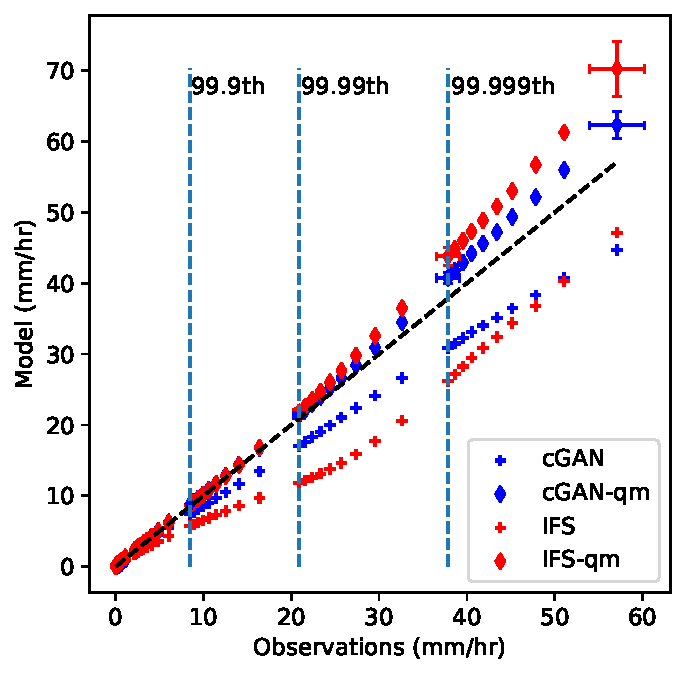
\includegraphics[width=\textwidth]{images/quantiles_total_final-nologs_217600.pdf}
         \caption{}
         \centering
     \end{subfigure}
     \hfill
     \begin{subfigure}[h]{0.5\textwidth}
         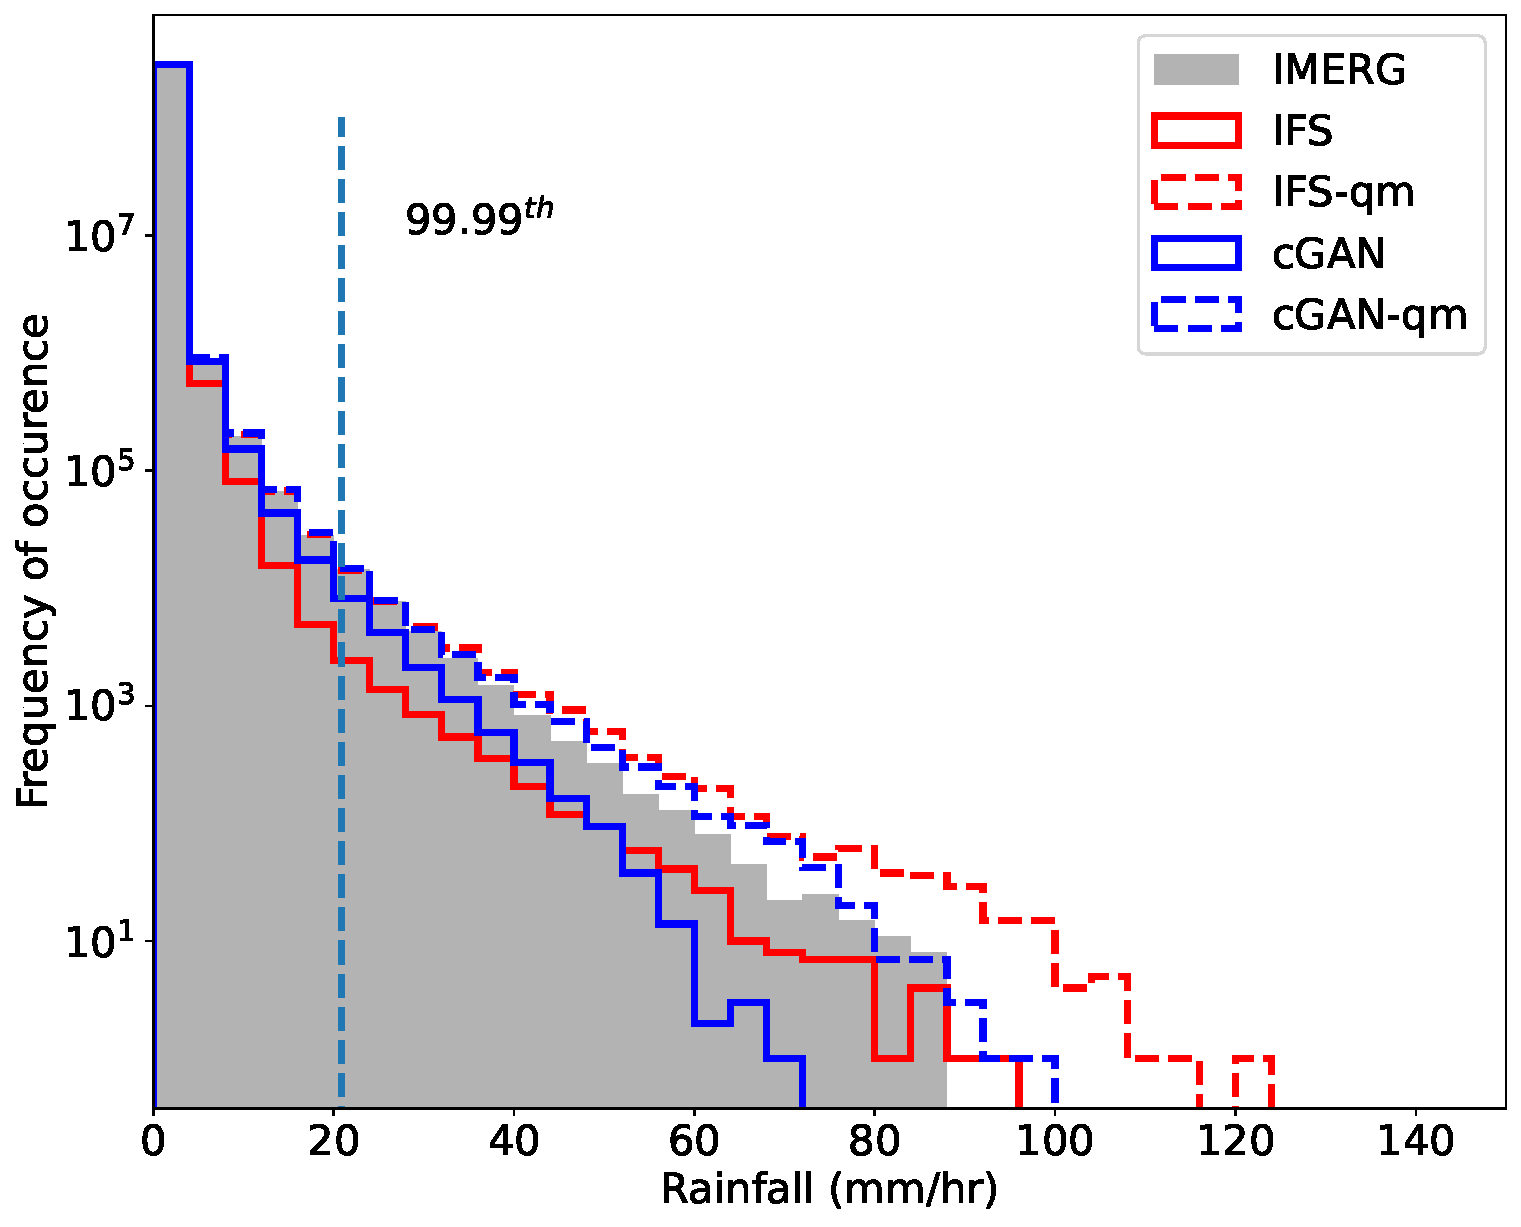
\includegraphics[width=\textwidth]{images/histograms_final-nologs_217600.pdf}
         \caption{}
        \centering
    \end{subfigure}
    \begin{subfigure}{0.48\textwidth}
     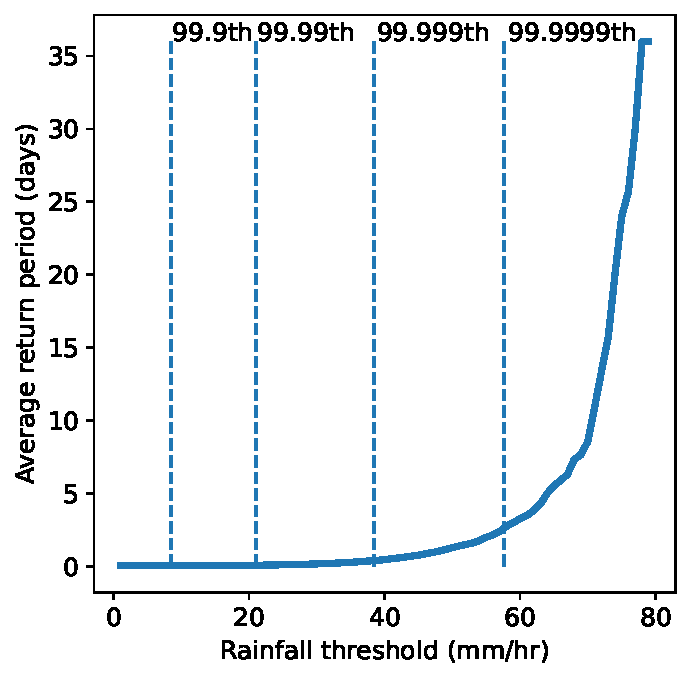
\includegraphics[width=\textwidth]{images/return_periods.pdf}
     \caption{}
     \end{subfigure}
     \centering
     \caption{a) Quantile-quantile plot, up to the $99.9999^{\text{th}}$ percentile. The black dashed line is the line along which a perfectly calibrated forecast would sit. The error bars indicate an estimate of 2 standard deviations from 1000 bootstrap samples b) A histogram showing the distribution of rainfall values; the vertical dashed blue line indicates the $99.99^{\text{th}}$ percentile of observed rainfall. The `qmap' suffix indicates that the forecast has been quantile mapped, as described in Sec.~\ref{subsec:qm}. c) The approximate return periods for different thresholds, calculated by finding the number of hours the threshold was exceeded for at least one pixel over the whole domain on the test set. The dashed lines indicating where the percentiles lie. }
     \label{fig:distribution}
\end{figure}

\begin{figure}[ht!]
     \centering
     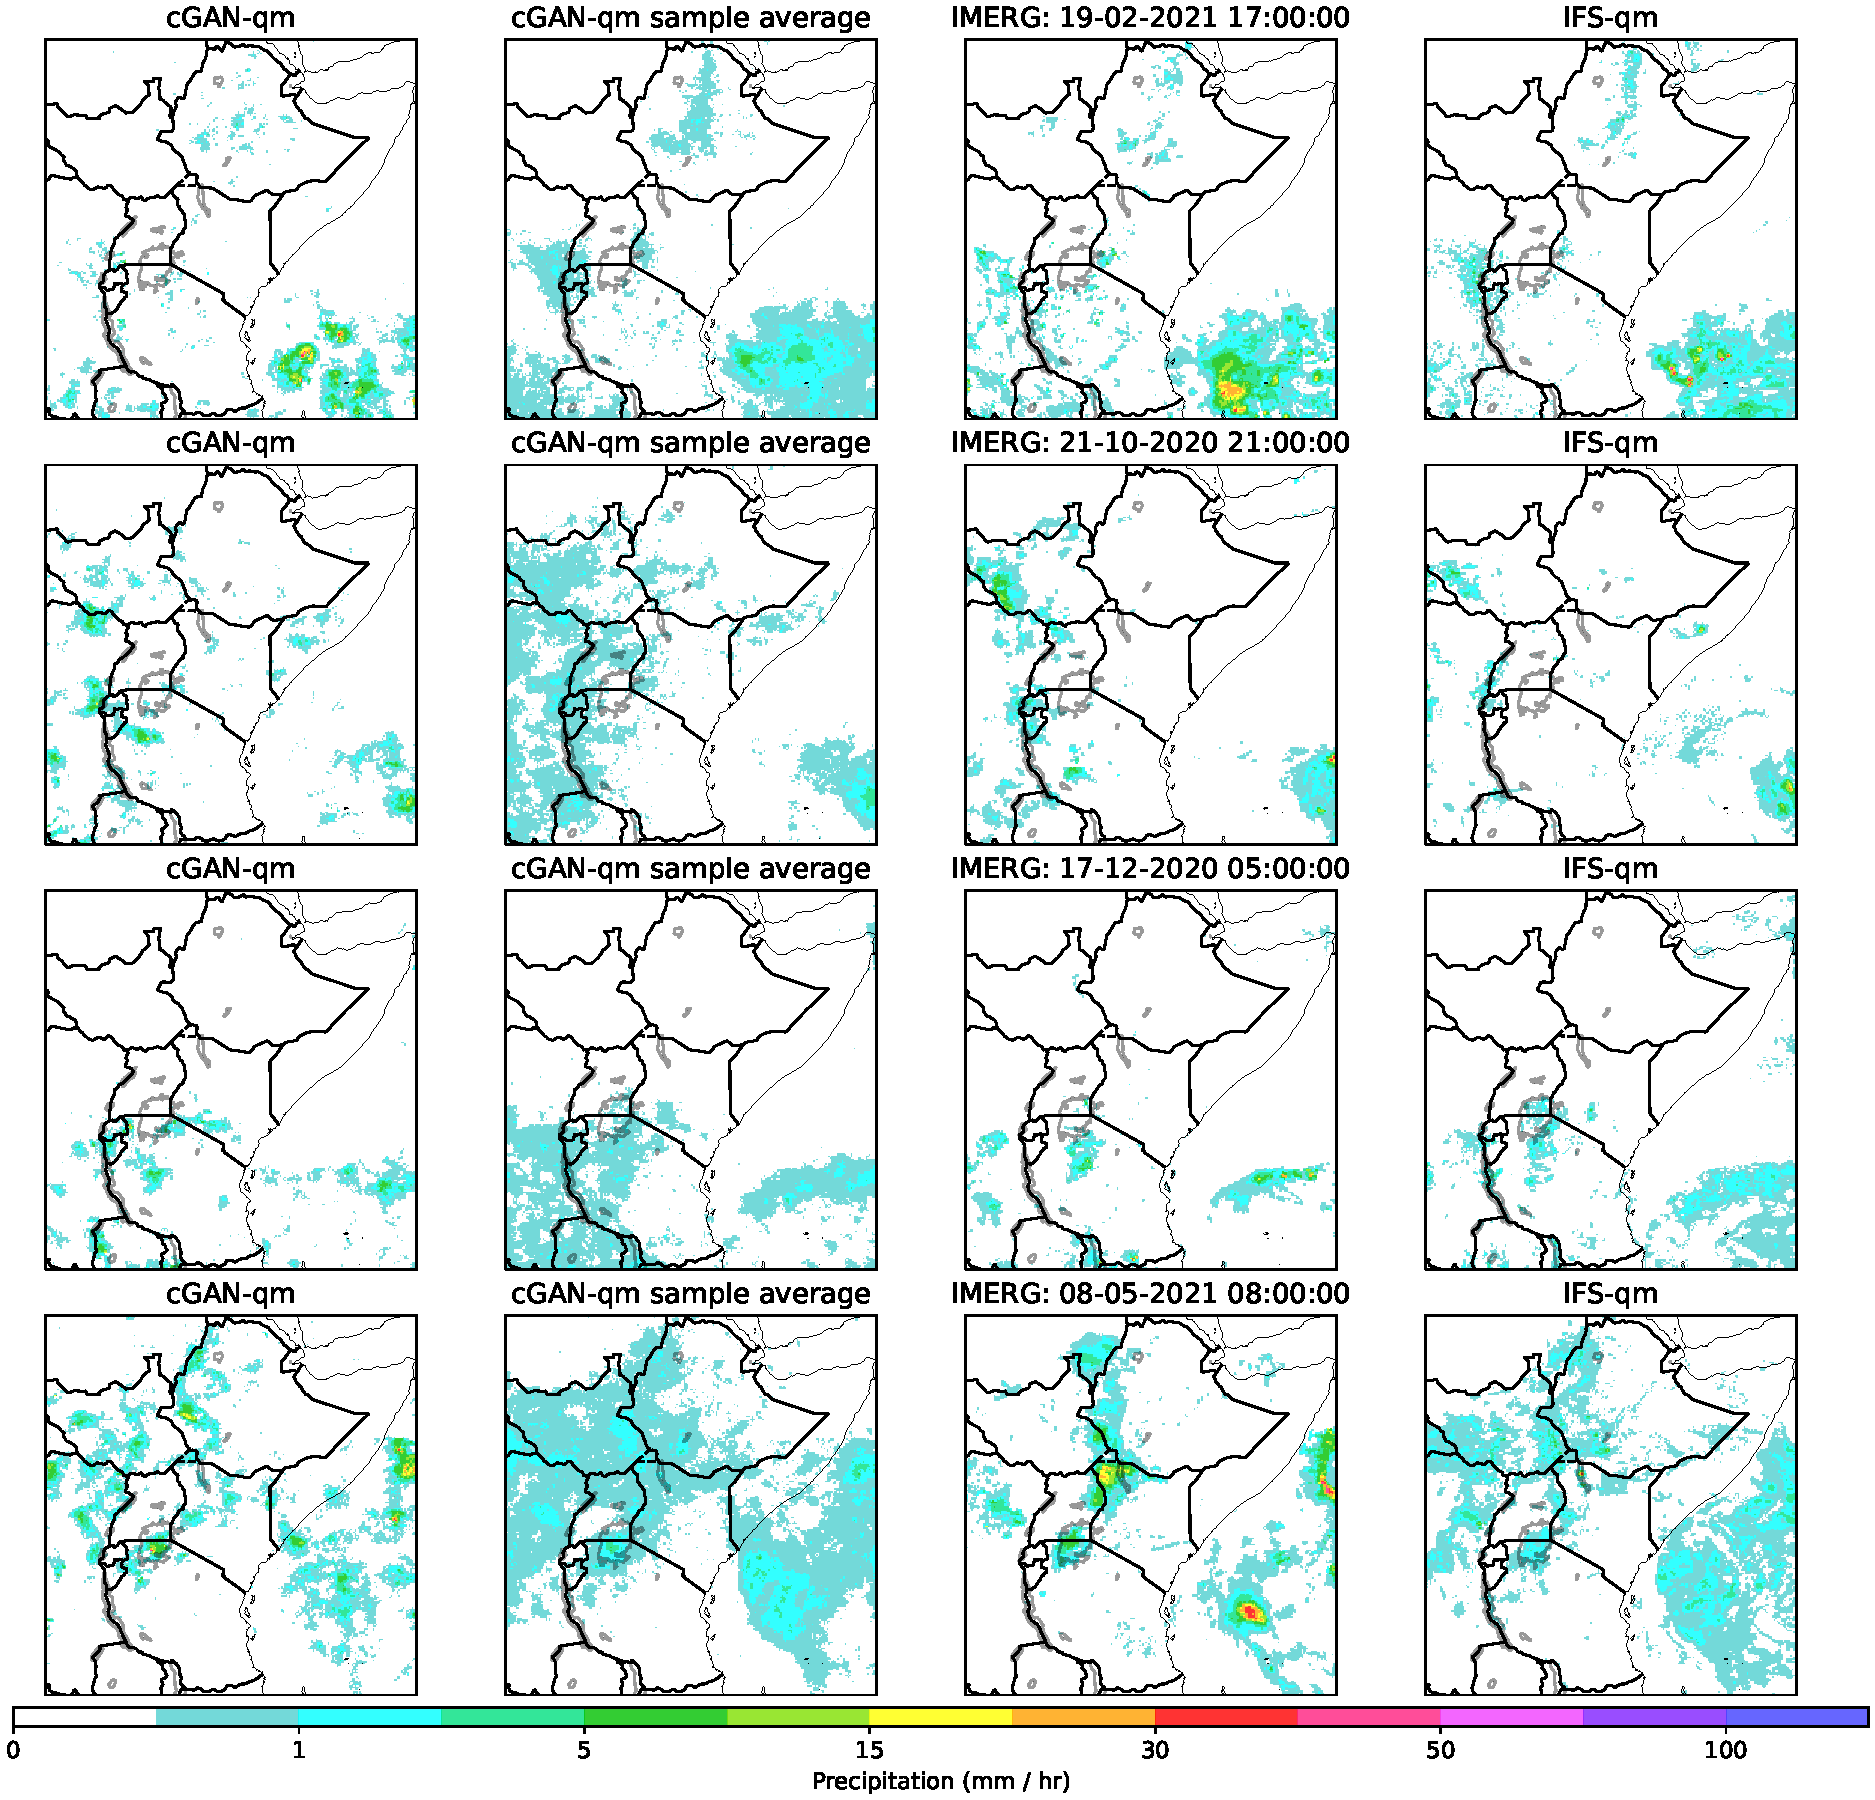
\includegraphics[width=1.05\textwidth]{images/cGAN_samples_IFS_final-nologs_217600.pdf}
     
     \caption{Example generated results from the cGAN-qm model, for a selection of hours throughout the test year, compared with IMERG observations and the IFS-qm model. Each row shows examples taken from the same timestamp. From left to right: a single member of the cGAN ensemble, the average of 20 cGAN-qm ensemble members, IMERG observations, the IFS forecast. }
     \label{fig:examples}
\end{figure}

\begin{figure}[!ht]
     \centering
     \begin{subfigure}{0.48\textwidth}
     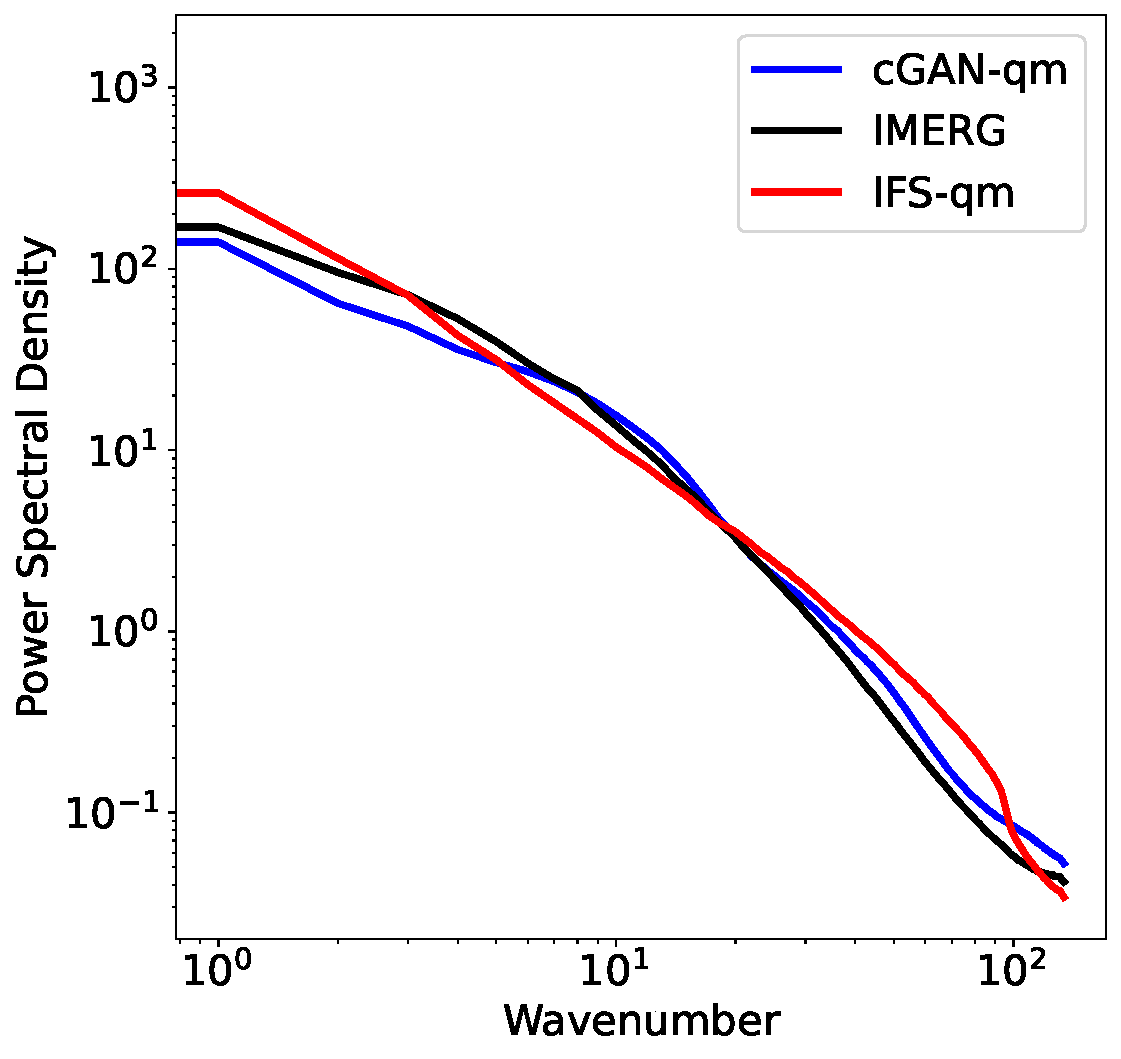
\includegraphics[width=\textwidth]{images/rapsd_final-nologs_217600.pdf}
     \caption{}
     \end{subfigure}
     
     \caption{a) Radially averaged power spectral density for the quantile mapped forecasts. 
}
     \label{fig:rapsd}
\end{figure}

\begin{figure}[!ht]
    \centering
    \begin{subfigure}{0.8\textwidth}
    \centering
     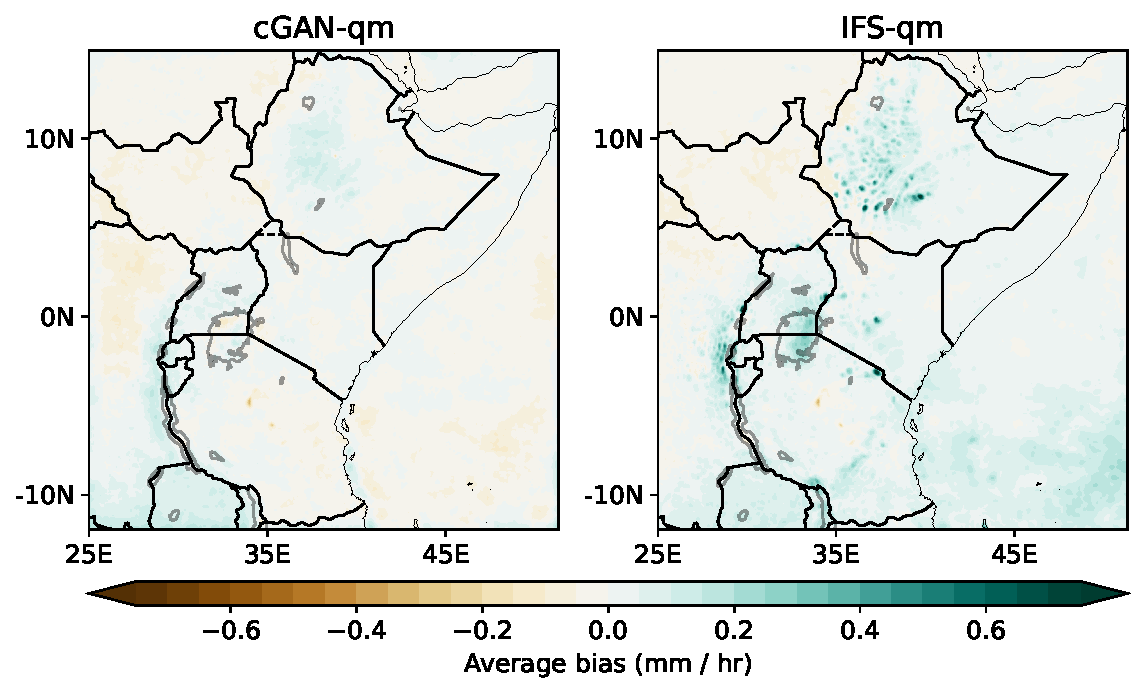
\includegraphics[width=\textwidth]{images/bias_final-nologs217600.pdf}
     \caption{}
     \end{subfigure}
     \begin{subfigure}{0.8\textwidth}
    \centering
     \includegraphics[width=\textwidth]{images/bias_std_final-nologs217600.pdf}
     \caption{}
     \end{subfigure}
    
     \caption{a) Average mean bias of the cGAN and IFS models b) Bias in the standard deviation for the cGAN-qm and IFS-qm models }
     \label{fig:bias}
\end{figure}

\begin{figure}
\centering
     \begin{subfigure}{\textwidth}
    \centering
     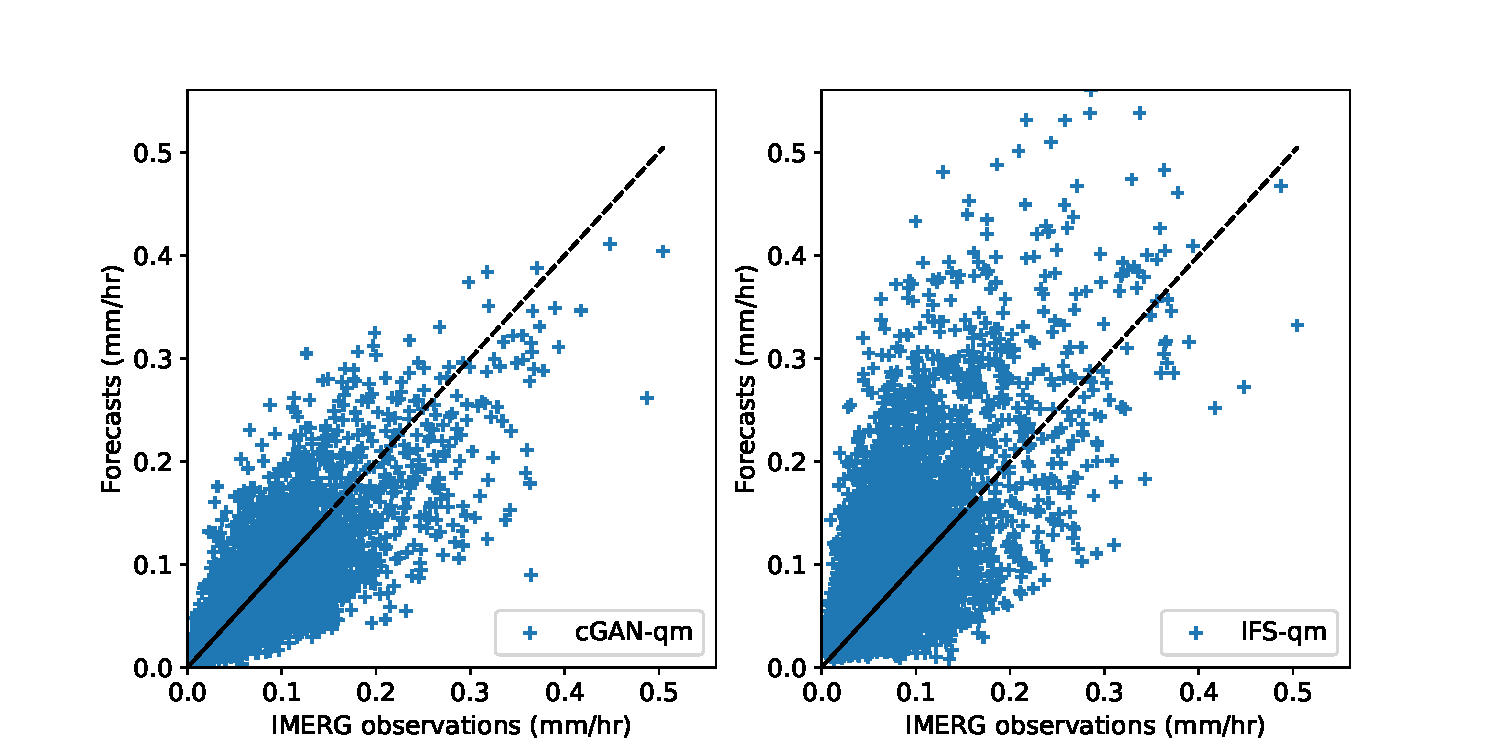
\includegraphics[width=\textwidth]{images/scatter_mean_final-nologs_217600.pdf}
     \caption{}
     \end{subfigure}
     \caption{Scatter plots of the domain averaged rainfall, for the IMERG observations against the cGAN-qm model (left) and IFS-qm model (right). In both plots the dashed black line represents the line that a perfect forecast would lie along. The Pearson correlation coefficient is 0.74 for the cGAN-qm model and 0.61 for the IFS data.}
     \label{fig:bias}
\end{figure}









\begin{figure}[t]
    \centering
     \begin{subfigure}[t]{0.33\textwidth}
 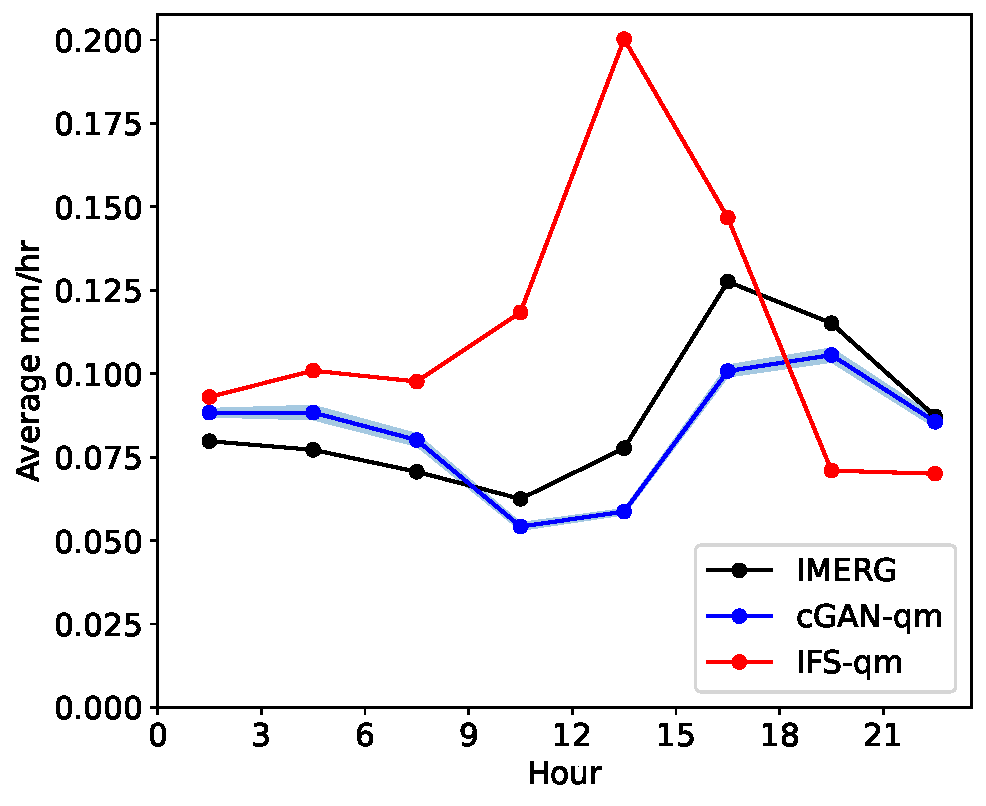
\includegraphics[width=\textwidth]{images/diurnal_cycle_mean_final-nologs_217600.pdf}
     \caption{}
     \end{subfigure}
     \begin{subfigure}[t]{0.32\textwidth}
     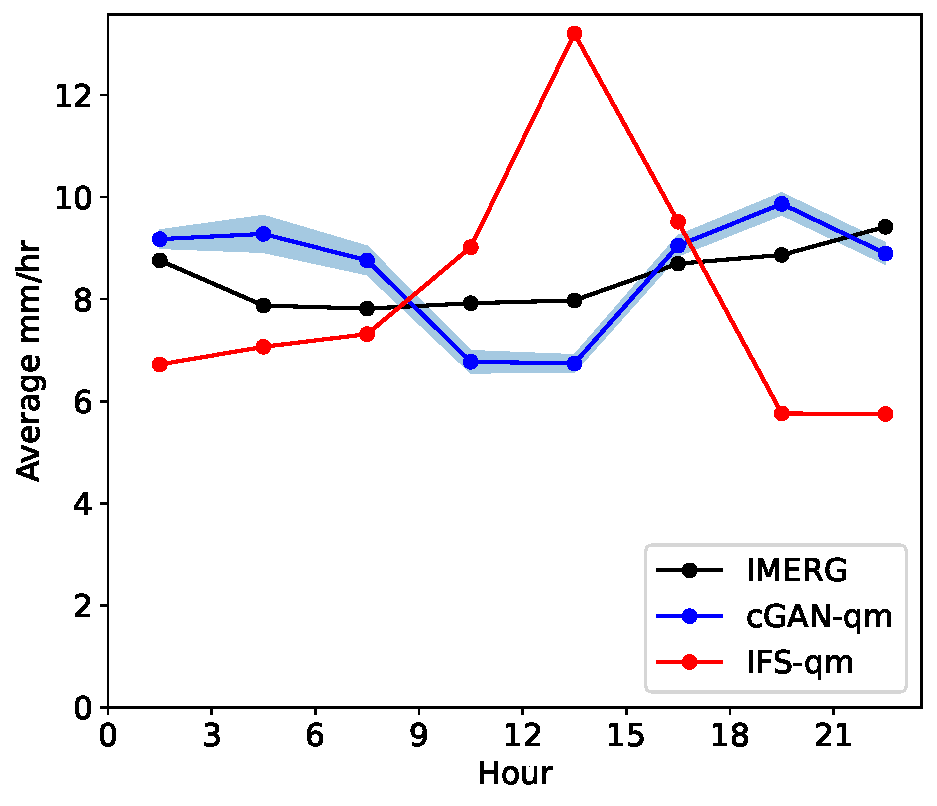
\includegraphics[width=\textwidth]{images/diurnal_cycle_quantile_999_final-nologs_217600.pdf}
     \caption{}
     \end{subfigure}
     \begin{subfigure}[t]{0.32\textwidth}
     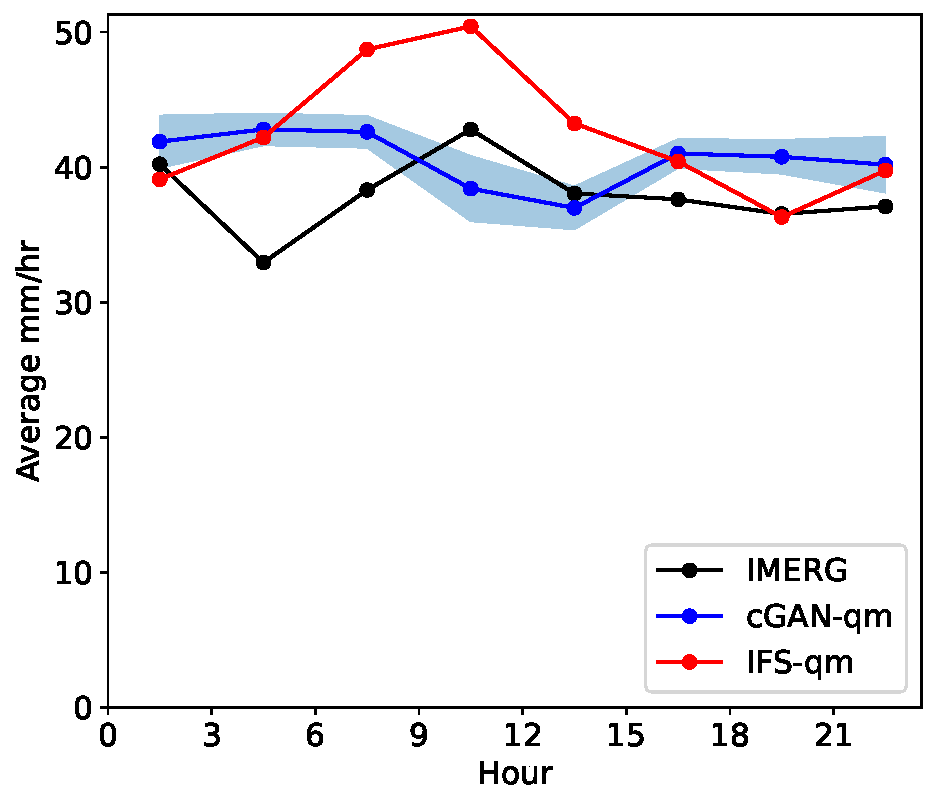
\includegraphics[width=\textwidth]{images/diurnal_cycle_quantile_99999_final-nologs_217600.pdf}
     \caption{}
     \end{subfigure}
     \caption{Evaluation of diurnal cycle in different summary statistics by hour (in local time) over the whole domain; a) mean rainfall, b) $99.9^{\text{th}}$ percentile, c) $99.999^{\text{th}}$ percentile. The shaded regions indicate $\pm2$ standard deviations about the mean. Note that rainfall at the $99.9^{\text{th}}$ percentile and above is mainly concentrated over Lake Victoria and over the sea.}
     \label{fig:diurnal}
\end{figure}

\begin{figure}[t]
\centering
\begin{subcaptionblock}{\textwidth}
        \centering
        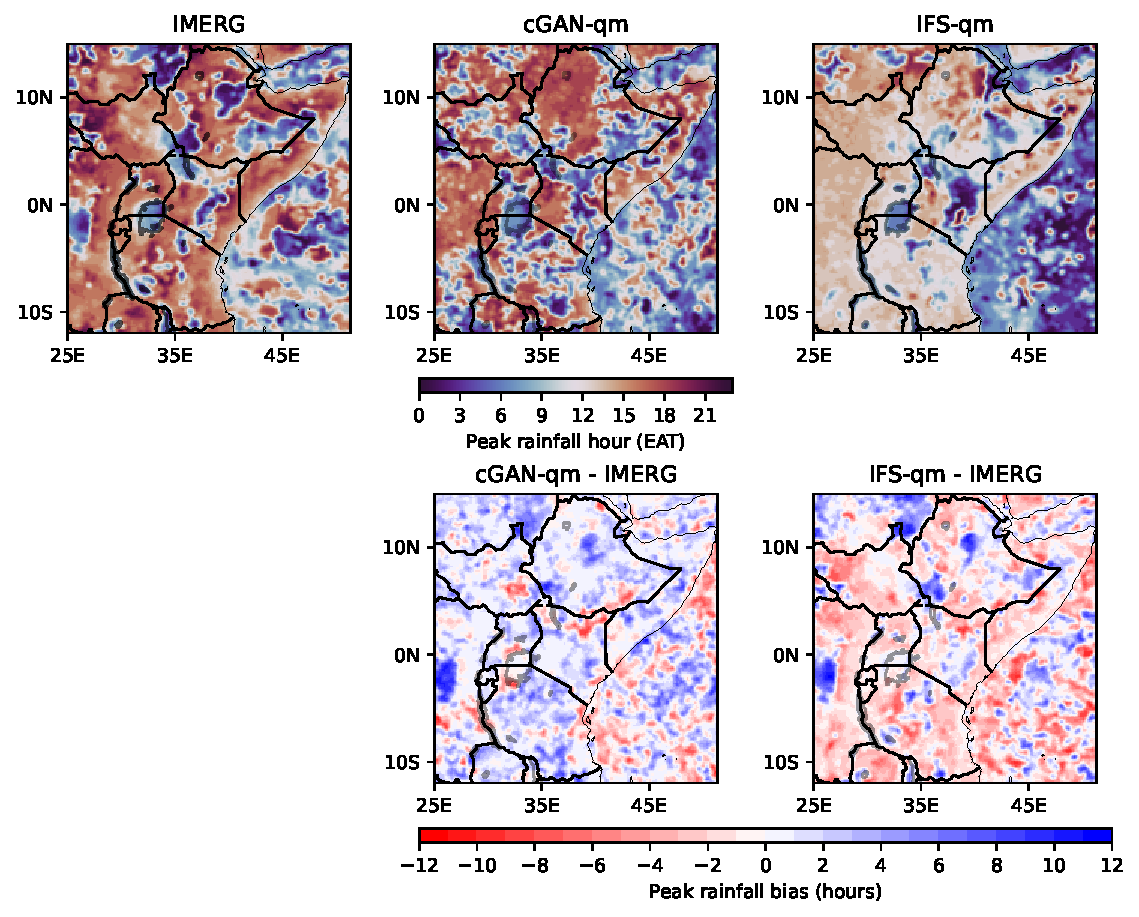
\includegraphics[width=\textwidth]{images/diurnal_cycle_map_All_final-nologs_217600.pdf}
        \caption{}\label{}
    \end{subcaptionblock}%
    \hfill
    % \begin{subcaptionblock}{\textwidth}
    %     \centering
    %     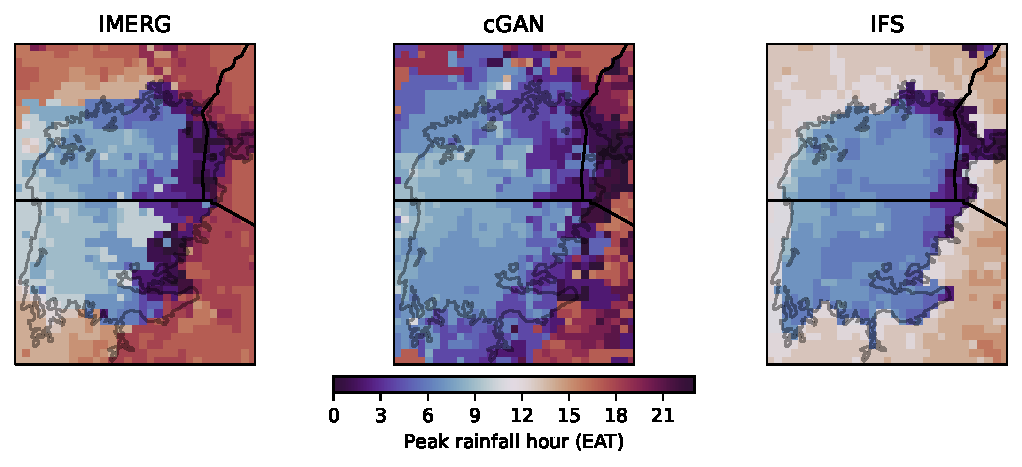
\includegraphics[width=\textwidth]{images/diurnal_cycle_map_Lake_Victoria_final-nologs_217600.pdf}
    %     \caption{}\label{}
    % \end{subcaptionblock}
     \caption{Map of peak rainfall hour averaged over the whole domain. A 3-hour moving average filter has been used to reduce noise in the time dimension before calculating the hour of peak rainfall.}
     \label{fig:peak_hour}
\end{figure}

 We first asses how well the forecasts capture the distribution of rainfall, by looking at a quantile-quantile plot and a histogram of rainfall distribution for 4000 samples taken from the test year, shown in Fig.~\ref{fig:distribution} (a) and (b) respectively. The raw model outputs are shown together with quantile-mapped outputs, indicated by a `-qm' suffix. From these we can see that the raw cGAN output is an improvement on the raw IFS output up to extremely high levels of rainfall (around 50mm/hr) beyond which point the IFS is closer to the distribution. Note that we wouldn't necessarily expect the GAN to align closely with the observed frequency distribution, since it is not explicitly trained to do so.

After both forecasts have been quantile mapped, they are much closer to the ideal line, with deviations at high quantiles which we attribute mainly to sampling variability. The scale of sampling variability was quantified by performing 1000 iterations of bootstrapping (see Sec.~\ref{sec:sample_var}) to estimate the standard deviation of the quantiles. These are shown in Fig.~\ref{fig:distribution}, where each error bar shows 2 standard deviations. It is likely that this is an underestimate of sampling variability, since there are correlations between samples that are unaccounted for, in which case it appears that the deviations of the quantiles from the diagonal is mainly due to sampling variability as expected. 


In order to also get a sense of how extreme these quantile values are, we plot the approximate return period in days for a range of thresholds in Fig.~\ref{fig:rapsd} (a), calculated over all hours in the test period. To calculate these, we find the total number of hours such that at least one point in the domain exceeds the threshold. Then the return period is estimated as the total number of hours in the test set, divided by the number of hours the threshold is exceeded. Finally this is divided by 24 to convert the answer to units of days. Note that due to correlations between hours, which artificially boost the number of times the threshold is exceeded, this will be a lower bound on the actual return period. Also note that the very high rainfall values (above around the $99.9^{\text{th}}$ percentile, $\sim20\text{mm/hr}$) are mainly concentrated over Lake Victoria and parts of the sea. 

Since these quantile mapped versions appear to much better forecasts, for the remaining diagnostics in this work we will focus on these quantile-mapped forecasts. Unless indicated otherwise, the following metrics are evaluated on a 4000 unique hours from the test period sampled uniformly over all dates from the test year.

We plot examples of the samples generated by the cGAN in Fig.~\ref{fig:examples}, for an ensemble size of 20. The generated samples appear to be fairly realistic, and the ensemble mean seems to correlate well with the locations and intensity of the observed rainfall. In the bottom row example (8am on 8th May 2021) we can see the cGAN removing some of the excess low rainfall seen over the land and see for the IFS-qm model. The top and bottom row examples also show both models not capturing the shape and maximum intensity of the high rainfall event occurring over the sea. To get a quantitative picture of how spatially realistic these rainfall patterns are, we plot the Radially Averaged Power Spectral Density (RAPSD) in Fig.~\ref{fig:rapsd}. From this we can that both quantile-mapped forecasts achieve similar results, with the cGAN slightly closer overall to the ideal line, and both forecasts showing opposite bias at the lowest wavenumbers, possibly due to sampling variability.

The plot of average bias in Fig.~\ref{fig:bias} (a) shows that on average the cGAN-qm under-predicts rainfall whilst the quantile-mapped IFS over-predicts. The cGAN also reduces the most prominent average biases of the IFS occurring over the Ethiopian highlands, Lake Victoria and the Western side of the East African rift, near Rwanda and Burundi. The effects on the bias in the standard deviation in Fig.~\ref{fig:bias} (b) are less obvious, there is some reduction in the sharpness of the peaks around the Ethiopian highlands, coastal regions and over the ocean, but there are also areas of increased negative bias in other parts of the ocean and in the western part of the domain over the Democratic Republic of Congo. The scatter plot in Fig.~\ref{fig:bias} shows how each model captures the domain-averaged rainfall; the cGAN-qm model is more tightly clustered around the ideal diagonal line, with the IFS-qm more spread out and tending to over-predict. This is reflected in the Pearson correlation coefficients; 0.74 for the cGAN-qm and 0.61 for the IFS-qm.



\begin{figure}[t]
    \centering
     \begin{subfigure}[t]{0.32\textwidth}
    \centering
 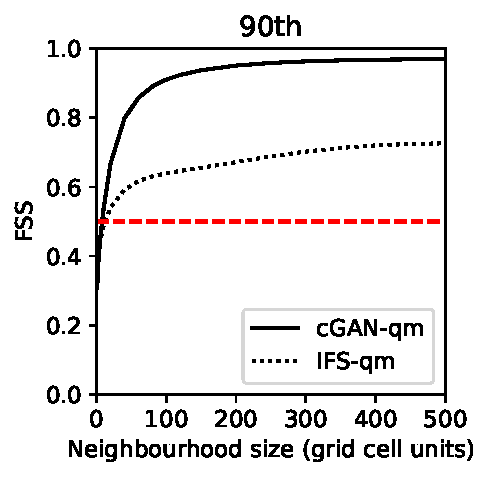
\includegraphics[width=\textwidth]{images/fss_q90th_final-nologs_217600.pdf}
     \caption{}
     \end{subfigure}
     \centering
     \begin{subfigure}[t]{0.32\textwidth}
     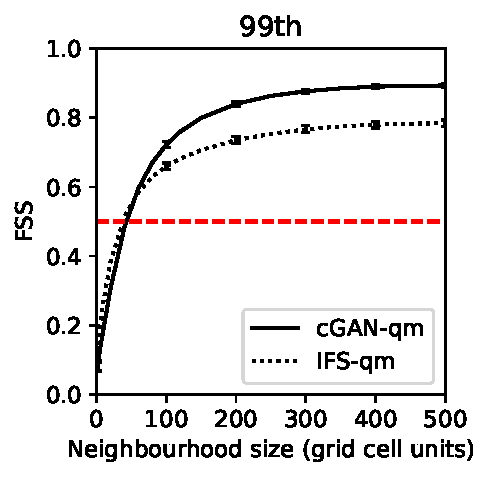
\includegraphics[width=\textwidth]{images/fss_q99th_final-nologs_217600.pdf}
     \caption{}
     \end{subfigure}
     \begin{subfigure}[t]{0.32\textwidth}
     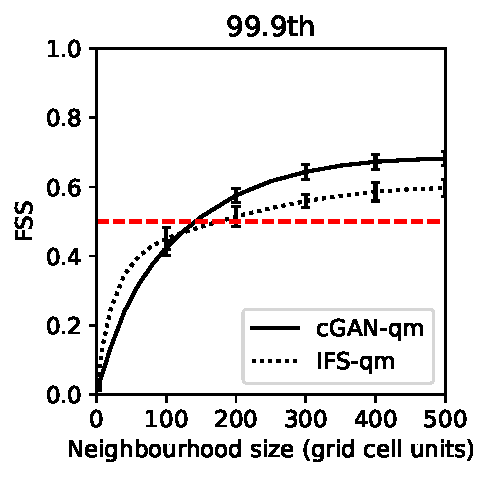
\includegraphics[width=\textwidth]{images/fss_q99.9th_final-nologs_217600.pdf}
     \caption{}
     \end{subfigure}
     \begin{subfigure}[t]{0.32\textwidth}
     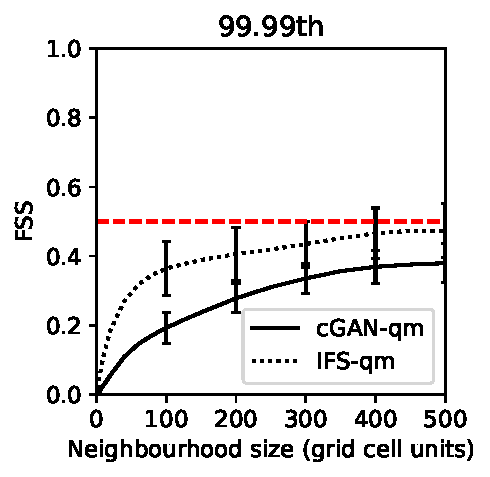
\includegraphics[width=\textwidth]{images/fss_q99.99th_final-nologs_217600.pdf}
     \caption{}
     \end{subfigure}
     \begin{subfigure}[t]{0.32\textwidth}
     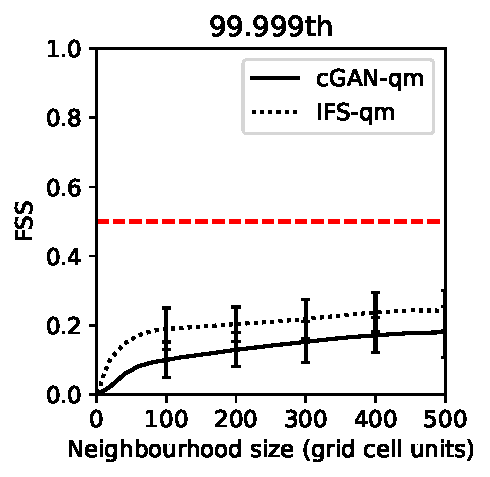
\includegraphics[width=\textwidth]{images/fss_q99.999th_final-nologs_217600.pdf}
     \caption{}
     \end{subfigure}
     \caption{Fractions Skill Score results for different quantile thresholds. The red dashed line indicates the `useful' criteria of 0.5 typically used to interpret this score. Error bars indicate $\pm2$ standard deviations estimated from bootstrapping with 50 samples. Note that rainfall at the $99.9^{\text{th}}$ percentile and above is mainly concentrated over Lake Victoria and over the sea. }
     \label{fig:fss}
\end{figure}

One source of error that the quantile mapping approach we use here is unable to adjust for is any bias in the diurnal cycle. Summary statistics of the rainfall as a function of hour are plotted in Fig.~\ref{fig:diurnal}, from which it is clear that the cGAN is making significant improvements to the diurnal cycle. The IFS forecast has a clear average bias around midday that is also prominent for high quantiles, whilst the cGAN is more aligned with observations.

We can gain insight into what regions are particularly driving this improvement from the plots of average peak rainfall hour in Fig.~\ref{fig:peak_hour}. The data is smoothed along the time axis using a centred moving average of length 3, in order to remove noise and make it easier to see any patterns in the data. The peak rainfall hour for the cGAN is fairly spatially noisy, but improvements can mainly be seen to occur on land. Note that the cGAN is not being given the hour as an input, but is instead using another variable as a proxy (e.g.~total incident solar radiation), which may explain the noisiness of the cGAN results. Looking at Lake Victoria, we can see that the cGAN correctly captures more of the nighttime maxima seen along the East coast of the lake and the morning maxima seen in the central and Western parts (see e.g.~\cite{woodhams_identifying_2019}), although it also tends to have a strong early bias in the land around the Western part of the lake.


\section{Event-based assessment}


We now look at how well each forecast is able to predict the occurrence of specific rainfall events, defined as the occurrence of rainfall above a certain threshold. In Fig.~\ref{fig:fss} we show plots of Fractions Skill Score (FSS) for different quantile thresholds, where the quantiles are calculated over the whole domain rather than for each grid cell individually (see Sec.~\ref{metrics:fss} for more details on the FSS). Estimated error bars are also shown, based on bootstrapping with 50 resamples (which we expect to be a lower bound since the effects of correlation in time are not taken into account). 

The value that the FSS reaches at the maximum neighbourhood size indicates the bias in the frequency with which forecasts exceed the particular rainfall threshold, and so we can see that, up to thresholds around the $99.9^{\text{th}}$ percentile, the cGAN has lower overall bias. Above this threshold, whilst the IFS shows higher results on average, the effects of sampling variability are significant (especially given these error bars are an underestimate), and so it is unclear whether the IFS is genuinely performing better or has just performed better on a specific event in the data. 

The FSS is typically interpreted relative to the `useful' criteria of $\frac{1}{2} + \frac{f_O}{2}$, and we can see that, for thresholds up to around the $99.9^{\text{th}}$ percentile the cGAN crosses this line at slightly lower neighbourhood size. However, as discussed in Sec.~\ref{metrics:fss}, it is known that skilful forecasts can lie below this line, and we can see that the IFS achieves higher scores at lower neighbourhood sizes, which suggests improved skill at fine resolutions. 

Overall then, these results suggest that, for up to around the $99.9^{\text{th}}$ percentile the cGAN scores better. Above this level the sampling variability in the test set makes it hard to draw any robust conclusions, but for this test set the IFS shows better performance on average at the very high percentiles.



\begin{figure}[ht]
    \centering
     \begin{subfigure}[t]{0.45\textwidth}

     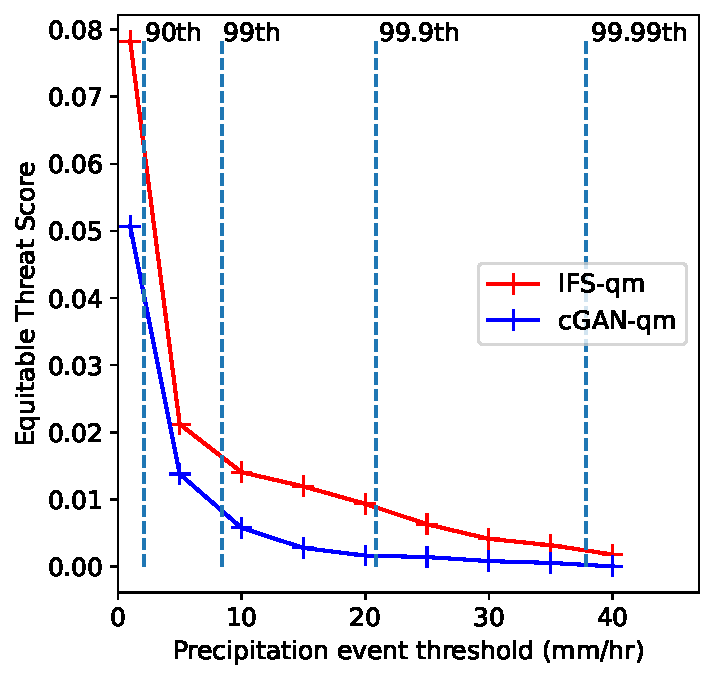
\includegraphics[width=\textwidth]{images/ets_final-nologs_217600.pdf}
     \caption{}
     \end{subfigure}
     \hfill
     \centering
     \begin{subfigure}[t]{0.49\textwidth}
     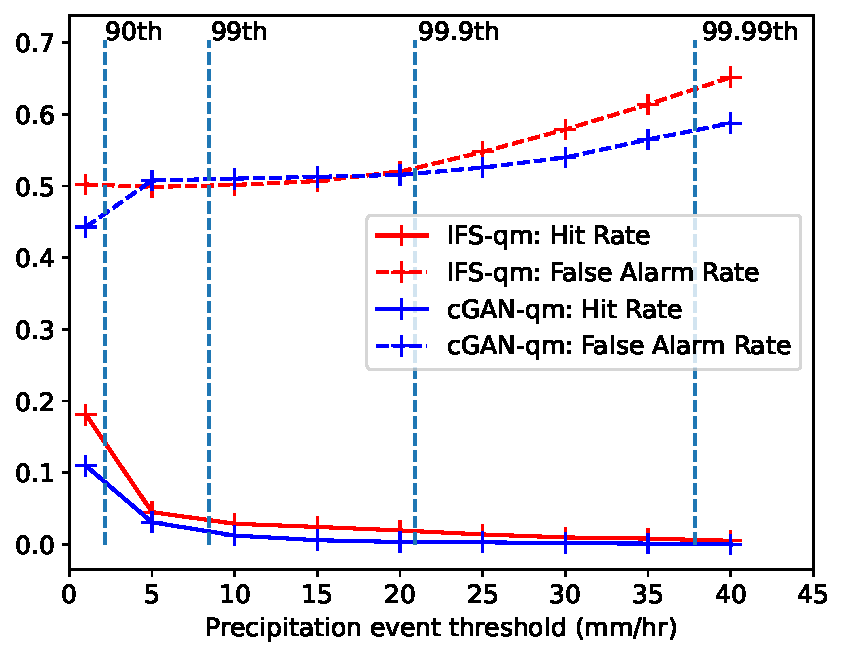
\includegraphics[width=\textwidth]{images/hit_rate_final-nologs_217600.pdf}
     \caption{}
     \end{subfigure}
     \caption{ a) Equitable threat score for the IFS-qm and cGAN-qm. b) Hit rate and False Alarm Rate for the IFS-qm and cGAN-qm models. Here an event is defined as whether not the rainfall at a particular grid cell exceed the rainfall threshold. Note that rainfall at the $99.9^{\text{th}}$ percentile and above is mainly concentrated over Lake Victoria and over the sea.}
     \label{fig:ets}
\end{figure}


The Equitable Threat score at several thresholds over the whole domain is shown in Fig.~\ref{fig:ets} (a), at the single pixel level. This shows that the quantile mapped IFS tends to perform better by this metric, which is in agreement with the FSS results that show the IFS performing better at smaller length scales. It is also perhaps to be expected from the quantile-mapped IFS forecast having a heavier-tailed rainfall distribution, as demonstrated in Fig.~\ref{fig:distribution}. In Fig~\ref{fig:ets} (b) the Hit Rate (HR) and False Alarm Rate (FAR) are shown, from which we can see that performance at low rainfall values is predominantly driven by differences in HR, and for extremely high values the FAR tends to increase significantly.



% [TOSO: SEDS scores are apparently better for rare events, according to ~\citep{wilson_forecast_2014}]
% [Also discriminant scores, such as KSS inform us how well the forecast distinguishes between positives and negatives, which is useful to a forecaster. ]

% TODO:
%     - Spread error 
%     quantile plots: Fcts -> IFS
% Bias plots: why is it -200% ? limit to +/- 20%. Green high / Brown low.

% mean bias and bias in standard deviation

% FSS: 90th percentile of rainy pixels?

% spread error: crosses 
% scatter plot: binned and maybe contoured? maybe domain averaged rainfall? or ensemble average?
% reliability?
% rank histogram?
        
\section{Assessment of ensemble calibration}


\begin{figure}[!ht]
    \centering
    \begin{subfigure}[t]{0.49\textwidth}
     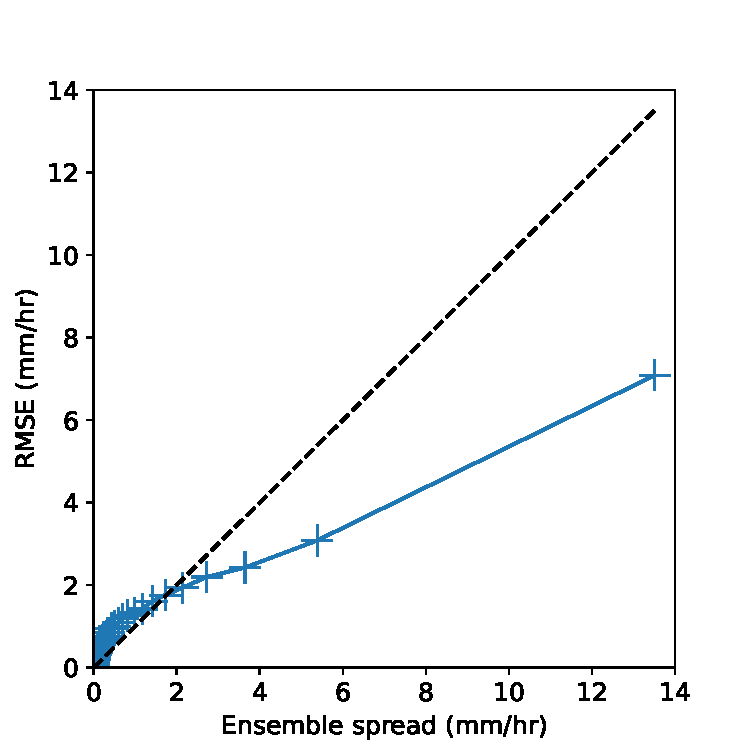
\includegraphics[width=\textwidth]{images/spread_error_final-nologs_217600.pdf}
     \caption{}
     \end{subfigure}
     \centering
    \begin{subfigure}[t]{0.49\textwidth}
     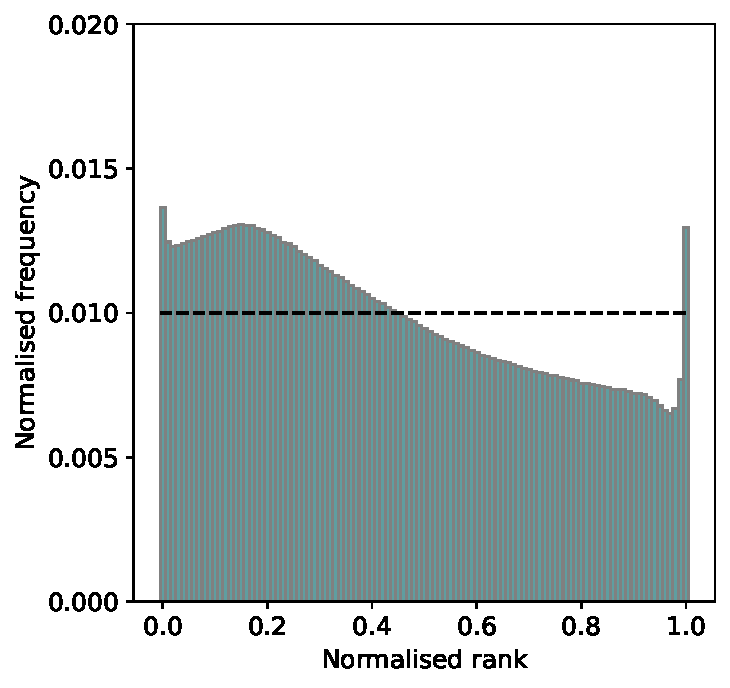
\includegraphics[width=\textwidth]{images/rank_hist_final-nologs_217600.pdf}
     \caption{}
     \end{subfigure}
     \centering
     \begin{subfigure}[t]{0.49\textwidth}
     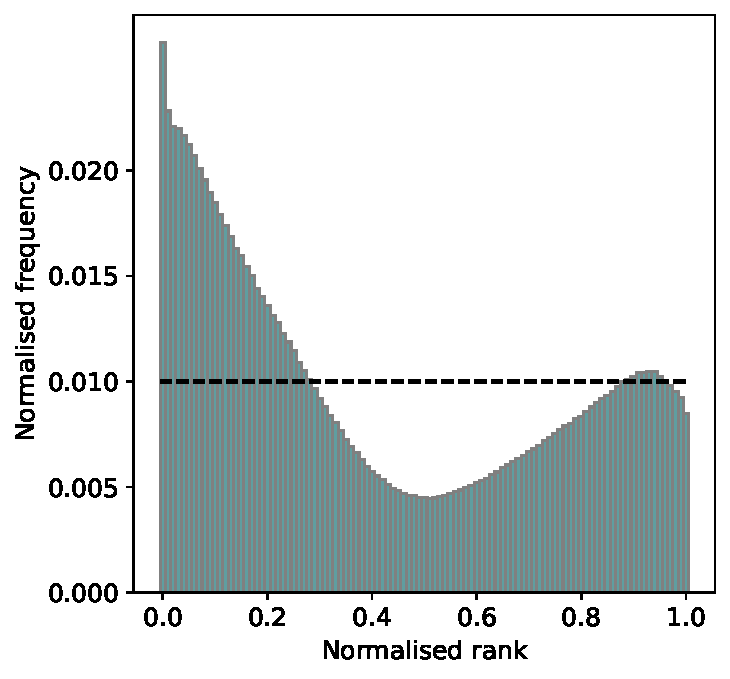
\includegraphics[width=\textwidth]{images/rank_hist_above_thr_final-nologs_217600.pdf}
     \caption{}
     \end{subfigure}
     \centering
      \begin{subfigure}[t]{0.49\textwidth}
     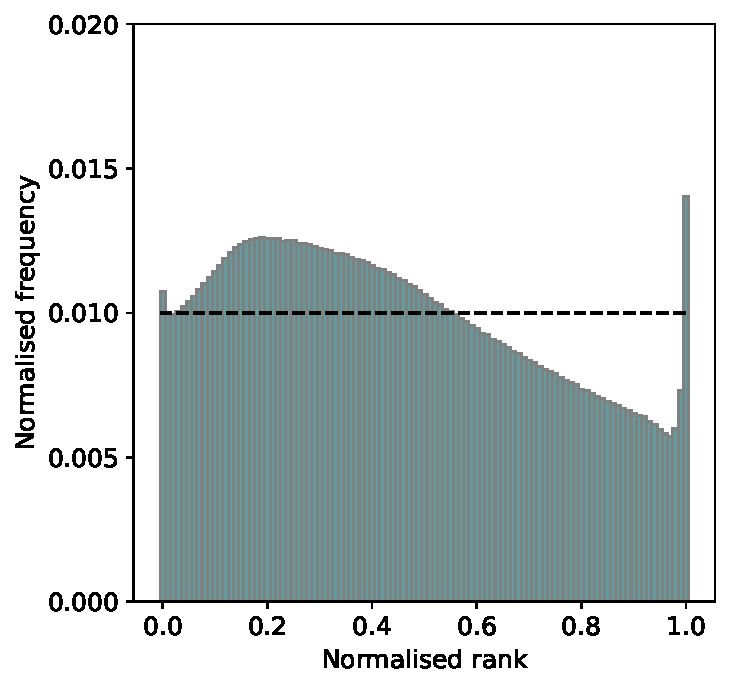
\includegraphics[width=\textwidth]{images/rank_hist_below_thr_final-nologs_217600.pdf}
     \caption{}
     \end{subfigure}
     
     
     \caption{Evaluation of the ensemble calibration of the cGAN, calculated using 500 samples of the cGAN with 100 ensemble members a) pixel-wise spread error, where the spread is split into 100 bins. b) pixel wise rank histogram, c) pixel wise rank histogram for pixels where the cGAN ensemble mean is $>0.1\text{mm/hr}$, c) pixel wise rank histogram for pixels where the cGAN ensemble mean is $\leq 0.1\text{mm/hr}$. For all plots, the dashed black line is the line that a perfectly calibrated ensemble would lie along. }
     \label{fig:ens_calib}
\end{figure}


We now focus on how well the cGAN ensemble is calibrated. Note that, as mentioned earlier in this chapter, one of our aims is to be able to convert a deterministic forecast into an ensemble forecast, so we do not have an ensemble forecast to compare with.

These results are assessed on 500 samples drawn uniformly over all days from the test year, each with 100 ensemble members. In Fig.~\ref{fig:ens_calib} (c) we show the spread error, where the spread is binned into 100 bins. From this we can see that the cGAN ensemble is slightly under-dispersive (i.e.~over-confident) for situations where there is low observed RMSE, but very over-dispersive (i.e.~under-confident) for situations where there is high RMSE. Since we would expect RMSE to roughly scale with the rainfall intensity, this suggests that the cGAN-qm model is over-confident at low rainfall values but under-confident at high rainfall values. Whilst the ensemble isn't calibrated perfectly, it is also reassuring to see that the cGAN has not fallen into the common failure mode of producing homogeneous images (which would produce extremely under-dispersive results).

The pixel-wise rank histogram in Fig.~\ref{fig:ens_calib} (b) also demonstrates that the ensemble deviates from the perfectly calibrated line, and appears to be made up of a mixture of behaviours (see Sec.~\ref{rank_hist} for more discussion of interpreting rank histograms). In general it is hard to uniquely attribute forecast behaviour from a rank histogram~\citep{hamill_interpretation_2001}; a U-shaped distribution can be indicative of under-dispersion of the ensemble, but can also be a mixture of over- and under-forecasting biases. 

In order to shed light on this, we also calculate rank histograms conditioned on the value in the cGAN-qm ensemble mean. In Fig.~\ref{fig:ens_calib} (c) and (d) we show rank histograms conditioned on the cGAN ensemble mean being $>0.1\text{mm/hr}$ and $\leq 0.1\text{mm/hr}$, respectively. In Fig.~\ref{fig:ens_calib} (c) we can see a clear U-shape for the high values, indicating under-dispersion, and a tendency to predict higher than the observations. From Fig.~\ref{fig:ens_calib} (d) we can see that the dominant behaviour at low rainfall intensity is over-prediction and over-dispersion. 

There is also an apparent contradiction between the spread-error plot result and the rank histogram: The spread-error plot appears to show decreasing dispersion with high rainfall values, while the rank histogram appears to show under-dispersion at high rainfall values. An explanation for this could be down to the fact that the rank histogram measures ordering and is insensitive to the particular error values, unlike the spread-error. Then potentially the spread-error is being skewed by a small number of forecasts that produce very high predictions, which doesn't show up on the rank histograms.

Another explanation for this contradiction is that, rather than being a U-shape indicating under-dispersion, the rank histogram in Fig.~\ref{fig:ens_calib} (c) is a mixture of systematic under- and over-forecasting, such that on average the cGAN over-forecasts, which also leads to large spreads.

    
% \section{Evaluation on extreme test set}

% ...


% A visual inspection of samples produced by the cGAN (Fig.~\ref{fig:cgan_sample}) confirms that it produces realistic spatial rainfall patterns; general features seem to be that the cGAN removes some of the wet bias at low intensities, and more accurately represent the high intensity rainfall. We use the radially-averaged spectral density as a measure of the spatial structure of the forecasts, shown in Fig.~\ref{fig:metrics}(a); this shows that the cGAN samples have a closer resemblance to the spectral density than the original forecast (although the cGAN tends to overpredict at high wavenumber - corresponding to smaller length scales). Compared to the quantile mapped forecast, the cGAN appears to do better at medium-range wavenumbers, but less well at higher wavenumbers. The cGAN also successfully corrects the position of the peak in diurnal cycle of the IFS (shown for the whole region in Fig.~\ref{fig:metrics}(c)), although it shows an overprediction in the peak height.

% Quantile-quantile plots reveal that the cGAN is able to correct the forecast bias up to the 99.99th percentile. However, beyond this there is extreme overprediction of high rainfall; this is an effect noted in~\citep{harris_generative_2022}, for which they introduced a rainfall threshold to cut off extremely high values. Also all the scores in~\citep{leinonen_stochastic_2020} were calculated after converting the rainfall to the range [0,1], and so any errors in intensity would not have registered in their analysis. A natural question to ask is why the discriminator in the GAN is unable to pick up on these extreme intensities; one explanation could be that GAN discriminators are known to be poor at learning for any frequency components in the image that have low magnitude (which in this case are the high frequency components)~\citep{schwarz_frequency_2021}. 

% note that the results capture the earlier peak rainfall in southeastern Lake Victoria, as mentioned in \citep{finney_implications_2019}.

\section{Conclusions}

In this chapter we have evaluated the cGAN model combined with quantile mapping (cGAN-qm) using a range of different metrics, aimed at assessing its performance at producing realistic spatial and temporal structure of precipitation, accurately forecasting events, and producing a well-calibrated ensemble. In order to provide a strong baseline, we used a neighbourhood quantile mapping technique applied to the IFS forecast. 

Quantile mapping was applied to the IFS forecast (IFS-qm) to provide a strong baseline, and also to the cGAN output in order to leverage the strengths of both quantile mapping and machine learning. With this baseline, the cGAN-qm and IFS-qm rainfall distributions are comparable, with both models tending to over-predict at high rainfall values (more than around 20mm/hr), although it is likely that much of this high quantile behaviour is due to sampling variability and the particular properties of the training and testing years. The cGAN-qm removes some of the biases in the IFS-qm model, as demonstrated by plots of the average bias and a scatter plot of domain averaged rainfall.

The most substantial improvement effect seen was for the diurnal cycle, which is known to be particularly problematic for conventional NWP models such as the IFS HRES to capture. The cGAN-qm model demonstrated a substantial improvement in the average diurnal cycle over the whole domain, which persisted when looking at the diurnal cycle of high quantiles. A map of peak rainfall intensity further demonstrated this, although there is still a significant amount of spatial noise in the cGAN peak rainfall hour, perhaps because time is not passed explicitly and the model has not yet learnt the full relationship between the variables and the diurnal cycle (and perhaps not all of the relevant variables are provided to enable it to do so).

To assess the ability of the model to predict events at a range of scales, the Fractions Skill Score (FSS) was used. Up to a high percentile ($99.9^{\text{th}}$) the cGAN-qm shows generally higher FSS scores, particularly at larger neighbourhood sizes, demonstrating that the cGAN-qm has lower bias in the frequency of pixels exceeding the threshold. For extremely high rainfall values, the IFS-qm forecast had a higher score although when sampling variability is taken into account this difference is not significant. To evaluate the ability of each forecast to predict rainfall events at individual points and times, without accounting for spatial structure, the Equitable Threat Score (ETS) was used; the IFS-qm model achieved higher ETS at all thresholds, although neither forecast demonstrated high enough scores to be considered usable.

The calibration of the cGAN ensemble was assessed via a spread-error plot and rank histograms. Both diagnostics indicate under-dispersion at high rainfall values and over-dispersion at lower rainfall values. This separation was partly identified through rank histograms conditioned on the ensemble mean being above or below a small threshold (01mm/hr).


Overall, these results highlights the subtlety in identifying the improvements a cGAN can bring; whilst the cGAN can significantly improve the raw IFS forecast, a strong baseline is crucial to find the areas where the cGAN can outperform conventional postprocessing methods. Compared to the quantile mapping baseline the improvements are mainly in the diurnal cycle and the skill scores for rainfall events at low to medium rainfall intensities. 




\ifSubfilesClassLoaded{%
    \bibliographystyle{alpha}
    \bibliography{references_z}

}{}


\end{document}